\section{Introduction}\label{introduction}

Since the invention of the computer in 1945, we have needed to translate
our thoughts into machine instructions. To solve a problem requiring a
computer, we must first find the solution and then translate this
solution into ``machine language.'' In order to overcome this
difficulty, a wide range of programming languages have been developed in
the last decade. Below, you can find a table with the different
categories of programming languages along with some examples, classified
subjectively into different levels of proximity to human language (Very
Low, Low, Moderate, Moderate to High, High, Very High). \textbar{}
Category \textbar{} Example \textbar{} Proximity to Human Language
\textbar{}
\textbar---------------------------------\textbar---------------------\textbar-----------------------------\textbar{}
\textbar{} Machine Languages \textbar{} Binary code \textbar{} Very Low
\textbar{} \textbar{} Assembly Languages \textbar{} x86 Assembly
\textbar{} Low \textbar{} \textbar{} Low-Level Programming Languages
\textbar{} C, C++ \textbar{} Moderate \textbar{} \textbar{} High-Level
Programming Languages\textbar{} Python, Java \textbar{} High \textbar{}
\textbar{} Very High-Level Programming Languages \textbar{} SQL, MATLAB
\textbar{} Very High \textbar{} \textbar{} Scripting Languages
\textbar{} JavaScript, PHP \textbar{} High \textbar{} \textbar{} Markup
Languages \textbar{} HTML, XML \textbar{} Moderate to High \textbar{}
\textbar{} Natural Language Programming \textbar{} Inform 7 \textbar{}
Very High \textbar{}

\begin{figure}
\centering
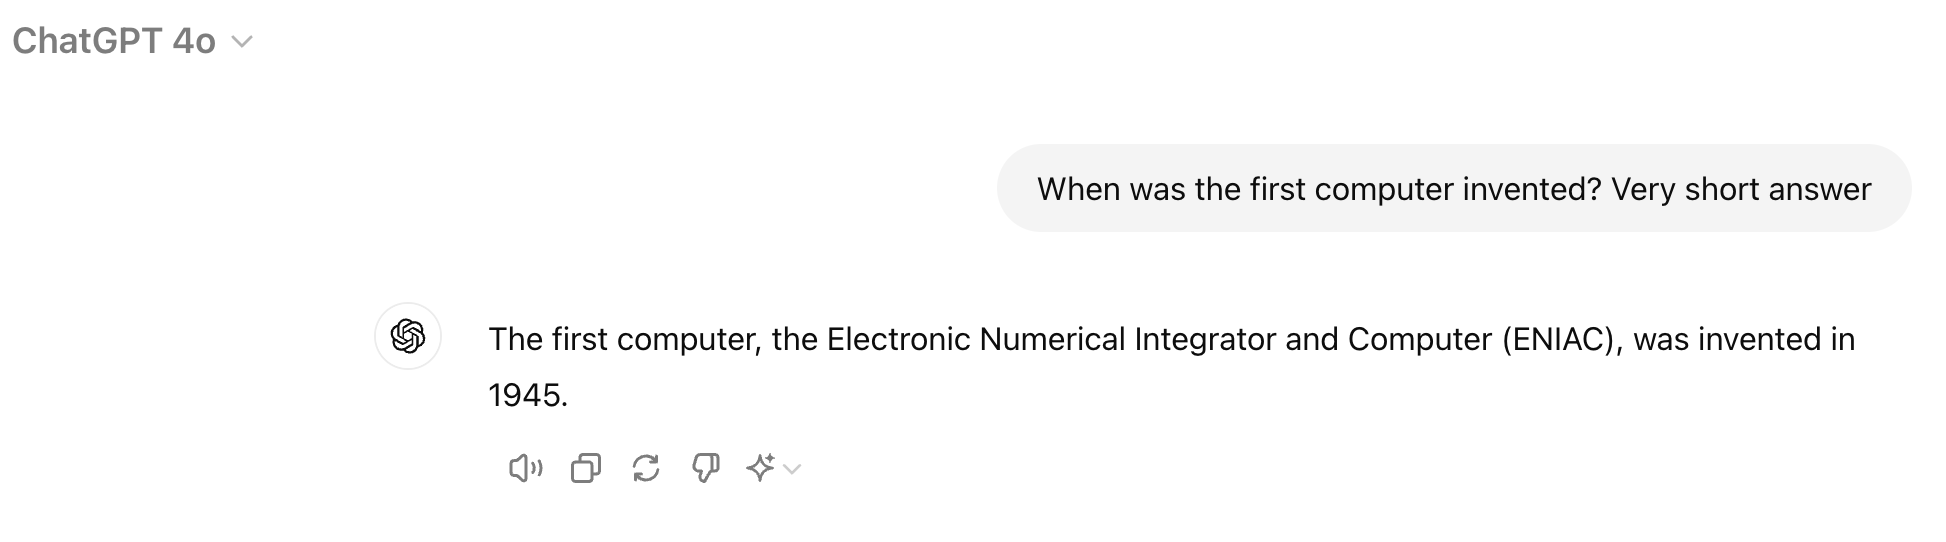
\includegraphics{images/first_computer.png}
\caption{first\_computer}
\end{figure}

So, could a machine understand natural language? This is the purpose of
a branch of Machine Learning known as Natural Language Processing (NLP).
NLP aims to minimize, even eliminate, the friction between humans and
computers. In words of the current Nvidia CEO Jensen Huang: ``It is our
job to create computing technology such that nobody has to program, and
that the programming language is human. Everybody in the world is now a
programmer. This is the miracle of Artificial Intelligence.'' This is a
strong and groundbreaking statement with which I partially agree.
Although I personally think that the role of Natural Language in this
context might be overestimated. The programmer's purpose nowadays is not
only to translate algorithms to machine language but also to actually
come up with these algorithms and sometimes, natural language is not
sufficient to express very complex ideas, which is why mathematics has
its own language.

\subsection{Data Extraction}\label{data-extraction}

One of the common tasks that it has gained relevance in the last decade
is data extraction. In the time of Big Data, Data Analysis and Data
Science extracting data from literally anywhere is crucial. NLP provides
a new tool to extract data which requires some understanding of Human
Language.

In this bachelor's thesis, we will use NLP to extract data from the
Boletín Oficial del Estado, which is the official gazette of Spain. The
number of pdfs published per month make incredibly difficult for an only
person to keep up with all the information (see graph below). LLMs
combined with a RAG system can very useful to retrieve information so it
can enhance transparency and accessibility to information. What is more,
\href{https://www.truelaw.ai/blog/legal-rag-vs-rag-a-technical-exploration-of-retrieval-systems}{it
is already being used in law firms}
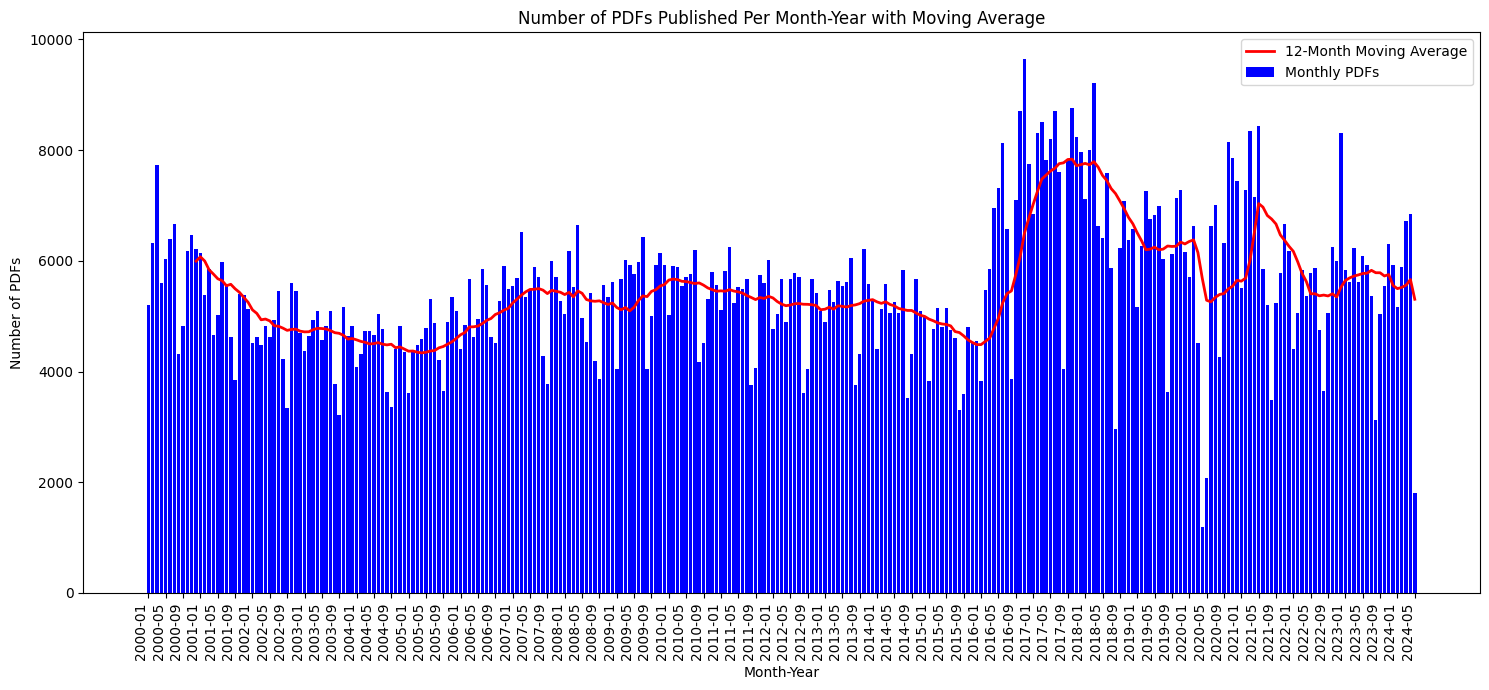
\includegraphics{images/pdfs_month.png} Image in
https://github.com/danmorper/NLP/blob/main/boe/xml.ipynb \# What is the
Boletín Oficial del Estado (BOE)? The Boletín Oficial del Estado (BOE)
is the official gazette of Spain, functioning as a daily publication
that serves as the official channel for disseminating legal norms,
regulations, and other important official announcements from the
government and other public bodies. The BOE is published every day and
made available in both PDF and XML formats. This allows for easy access
and verification of legal documents by citizens, organizations, and
legal entities.

Here is a general schema of how BOE XML files are structured: \#\#
Structure of BOE XML Files

\begin{Shaded}
\begin{Highlighting}[]
\VariableTok{Sumario}
\OperatorTok{|}
\OperatorTok{|}\CommentTok{{-}{-} Meta}
\OperatorTok{|}   \OperatorTok{|}\CommentTok{{-}{-} pub}
\OperatorTok{|}   \OperatorTok{|}\CommentTok{{-}{-} ano}
\OperatorTok{|}   \OperatorTok{|}\CommentTok{{-}{-} fecha}
\OperatorTok{|}   \OperatorTok{|}\CommentTok{{-}{-} fechaInv}
\OperatorTok{|}   \OperatorTok{|}\CommentTok{{-}{-} fechaAnt}
\OperatorTok{|}   \OperatorTok{|}\CommentTok{{-}{-} fechaAntAnt}
\OperatorTok{|}   \OperatorTok{|}\CommentTok{{-}{-} fechaSig}
\OperatorTok{|}   \OperatorTok{|}\CommentTok{{-}{-} fechaPub}
\OperatorTok{|}   \OperatorTok{|}\CommentTok{{-}{-} pubDate}
\OperatorTok{|}
\OperatorTok{|}\CommentTok{{-}{-} diario (nbo)}
\OperatorTok{|}   \OperatorTok{|}\CommentTok{{-}{-} sumario\_nbo (id)}
\OperatorTok{|}   \OperatorTok{|}   \OperatorTok{|}\CommentTok{{-}{-} urlPdf (szBytes, szKBytes)}
\OperatorTok{|}   \OperatorTok{|}
\OperatorTok{|}   \OperatorTok{|}\CommentTok{{-}{-} seccion (num, nombre)}
\OperatorTok{|}       \OperatorTok{|}\CommentTok{{-}{-} departamento (nombre, etq)}
\OperatorTok{|}           \OperatorTok{|}\CommentTok{{-}{-} item (id)}
\OperatorTok{|}               \OperatorTok{|}\CommentTok{{-}{-} urlPdf}
\OperatorTok{|}               \OperatorTok{|}\CommentTok{{-}{-} urlHtm}
\OperatorTok{|}               \OperatorTok{|}\CommentTok{{-}{-} urlXml}
\end{Highlighting}
\end{Shaded}

\section{Principal Component Analysis
(PCA)}\label{principal-component-analysis-pca}

{[} X =

\begin{pmatrix} 
x_{1.} \\ 
\vdots \\ 
x_{n.}
\end{pmatrix} 
\quad \implies \quad

X \in \mathbb{R}\^{}\{n \times p\} {]}

Only assumption on \(X\) is that its mean vector and covariance matrix
exist.

Let \(\delta = (\delta_1, \ldots, \delta_p)'\) be called the weighting
vector. Then the weighted average is: {[} \delta' X =
\sum\_\{j=1\}\^{}\{p\} \delta\emph{j X\_j \quad \text{such that}
\quad \sum}\{j=1\}\^{}\{p\} \delta\_j = 1 {]}

In order to properly choose \(\delta\), we will maximize the variance:
{[} \max\emph{\{\delta \in M\} \text{Var}(\delta' X) =
\max}\{\delta \in M\} \delta' \text{Var}(X) \delta  {]} {[} M =
\{\delta : \textbar{}\delta\textbar{} = 1\} {]}

We call \(\Sigma = \text{Var}(X)\).

{[} \max\_\{\delta \in M\} \delta' \Sigma \delta  {]}

This is a quadratic convex maximization problem with nonlinear
constraints.

{[} \mathcal{L} (\delta, \lambda) = \delta' \Sigma \delta -
\lambda (\delta' \delta - 1) {]}

\begin{itemize}
\item
  \(\nabla_{\delta} \mathcal{L} = 0 : \Sigma \delta = \lambda \delta\)
\item
  \(\lambda\): eigenvalue
\item
  \(\delta\): eigenvector of \(\lambda\)
\item
  \(\delta' \Sigma \delta = \lambda \delta' \delta = \lambda\)
\end{itemize}

Thus, {[} \max\_\{\delta\} \lambda \quad \text{subject to}
\quad \Sigma \delta = \lambda \delta, \textbar{}\delta\textbar{} = 1 {]}
So we call \(\delta\) the first principal component.

Let \(\delta^1, \ldots, \delta^j\) fit \(j\) principal components. The
\(j+1\) principal component is the result of: {[} \max \delta'
\Sigma \delta  {]} subject to {[} \delta' \delta\^{}i = 0
\quad \forall i \in \{1, \ldots, j\} {]} {[} \delta' \delta = 1 {]}

The \(j\)-th principal component is an eigenvector associated to the
\(j\)-th eigenvalue of \(\Sigma\).

\begin{Shaded}
\begin{Highlighting}[]
\ImportTok{import}\NormalTok{ numpy }\ImportTok{as}\NormalTok{ np}
\ImportTok{import}\NormalTok{ pandas }\ImportTok{as}\NormalTok{ pd}
\ImportTok{import}\NormalTok{ matplotlib.pyplot }\ImportTok{as}\NormalTok{ plt}
\ImportTok{from}\NormalTok{ mpl\_toolkits.mplot3d }\ImportTok{import}\NormalTok{ Axes3D}
\ImportTok{from}\NormalTok{ sklearn.preprocessing }\ImportTok{import}\NormalTok{ StandardScaler}

\CommentTok{\# Create a sample dataset in 3 dimensions}
\NormalTok{np.random.seed(}\DecValTok{42}\NormalTok{)}
\NormalTok{mean }\OperatorTok{=}\NormalTok{ [}\DecValTok{0}\NormalTok{, }\DecValTok{0}\NormalTok{, }\DecValTok{0}\NormalTok{]}
\NormalTok{cov }\OperatorTok{=}\NormalTok{ [[}\DecValTok{1}\NormalTok{, }\FloatTok{0.8}\NormalTok{, }\FloatTok{0.5}\NormalTok{], [}\FloatTok{0.8}\NormalTok{, }\DecValTok{1}\NormalTok{, }\FloatTok{0.3}\NormalTok{], [}\FloatTok{0.5}\NormalTok{, }\FloatTok{0.3}\NormalTok{, }\DecValTok{1}\NormalTok{]]  }\CommentTok{\# covariance matrix}
\NormalTok{data }\OperatorTok{=}\NormalTok{ np.random.multivariate\_normal(mean, cov, }\DecValTok{100}\NormalTok{)}
\NormalTok{df }\OperatorTok{=}\NormalTok{ pd.DataFrame(data, columns}\OperatorTok{=}\NormalTok{[}\StringTok{\textquotesingle{}Feature\_1\textquotesingle{}}\NormalTok{, }\StringTok{\textquotesingle{}Feature\_2\textquotesingle{}}\NormalTok{, }\StringTok{\textquotesingle{}Feature\_3\textquotesingle{}}\NormalTok{])}

\CommentTok{\# Standardize the data}
\NormalTok{scaler }\OperatorTok{=}\NormalTok{ StandardScaler()}
\NormalTok{scaled\_data }\OperatorTok{=}\NormalTok{ scaler.fit\_transform(df)}

\CommentTok{\# Calculate the covariance matrix manually}
\NormalTok{cov\_matrix }\OperatorTok{=}\NormalTok{ np.cov(scaled\_data, rowvar}\OperatorTok{=}\VariableTok{False}\NormalTok{)}
\BuiltInTok{print}\NormalTok{(}\StringTok{"Covariance Matrix:"}\NormalTok{)}
\BuiltInTok{print}\NormalTok{(cov\_matrix)}

\CommentTok{\# Perform eigenvalue and eigenvector decomposition}
\NormalTok{eigenvalues, eigenvectors }\OperatorTok{=}\NormalTok{ np.linalg.eigh(cov\_matrix)}
\BuiltInTok{print}\NormalTok{(}\StringTok{"Eigenvalues:"}\NormalTok{)}
\BuiltInTok{print}\NormalTok{(eigenvalues)}
\BuiltInTok{print}\NormalTok{(}\StringTok{"Eigenvectors:"}\NormalTok{)}
\BuiltInTok{print}\NormalTok{(eigenvectors)}

\CommentTok{\# Sort the eigenvalues and eigenvectors in descending order}
\NormalTok{idx }\OperatorTok{=}\NormalTok{ np.argsort(eigenvalues)[::}\OperatorTok{{-}}\DecValTok{1}\NormalTok{]}
\NormalTok{eigenvalues }\OperatorTok{=}\NormalTok{ eigenvalues[idx]}
\NormalTok{eigenvectors }\OperatorTok{=}\NormalTok{ eigenvectors[:, idx]}

\CommentTok{\# Transform the data to the principal components}
\NormalTok{pca\_result }\OperatorTok{=}\NormalTok{ np.dot(scaled\_data, eigenvectors)}
\NormalTok{pca\_df }\OperatorTok{=}\NormalTok{ pd.DataFrame(pca\_result, columns}\OperatorTok{=}\NormalTok{[}\StringTok{\textquotesingle{}PC1\textquotesingle{}}\NormalTok{, }\StringTok{\textquotesingle{}PC2\textquotesingle{}}\NormalTok{, }\StringTok{\textquotesingle{}PC3\textquotesingle{}}\NormalTok{])}

\CommentTok{\# Plot the original data in 3D}
\NormalTok{fig }\OperatorTok{=}\NormalTok{ plt.figure(figsize}\OperatorTok{=}\NormalTok{(}\DecValTok{12}\NormalTok{, }\DecValTok{6}\NormalTok{))}
\NormalTok{ax }\OperatorTok{=}\NormalTok{ fig.add\_subplot(}\DecValTok{121}\NormalTok{, projection}\OperatorTok{=}\StringTok{\textquotesingle{}3d\textquotesingle{}}\NormalTok{)}
\NormalTok{ax.scatter(df[}\StringTok{\textquotesingle{}Feature\_1\textquotesingle{}}\NormalTok{], df[}\StringTok{\textquotesingle{}Feature\_2\textquotesingle{}}\NormalTok{], df[}\StringTok{\textquotesingle{}Feature\_3\textquotesingle{}}\NormalTok{])}
\NormalTok{ax.set\_xlabel(}\StringTok{\textquotesingle{}Feature 1\textquotesingle{}}\NormalTok{)}
\NormalTok{ax.set\_ylabel(}\StringTok{\textquotesingle{}Feature 2\textquotesingle{}}\NormalTok{)}
\NormalTok{ax.set\_zlabel(}\StringTok{\textquotesingle{}Feature 3\textquotesingle{}}\NormalTok{)}
\NormalTok{ax.set\_title(}\StringTok{\textquotesingle{}Original Data in 3D\textquotesingle{}}\NormalTok{)}

\CommentTok{\# Plot the principal components in 3D}
\NormalTok{ax }\OperatorTok{=}\NormalTok{ fig.add\_subplot(}\DecValTok{122}\NormalTok{, projection}\OperatorTok{=}\StringTok{\textquotesingle{}3d\textquotesingle{}}\NormalTok{)}
\NormalTok{ax.scatter(pca\_df[}\StringTok{\textquotesingle{}PC1\textquotesingle{}}\NormalTok{], pca\_df[}\StringTok{\textquotesingle{}PC2\textquotesingle{}}\NormalTok{], pca\_df[}\StringTok{\textquotesingle{}PC3\textquotesingle{}}\NormalTok{])}
\ControlFlowTok{for}\NormalTok{ i }\KeywordTok{in} \BuiltInTok{range}\NormalTok{(}\BuiltInTok{len}\NormalTok{(eigenvectors)):}
\NormalTok{    vector }\OperatorTok{=}\NormalTok{ eigenvectors[:, i] }\OperatorTok{*}\NormalTok{ np.sqrt(eigenvalues[i])}
\NormalTok{    ax.quiver(}\DecValTok{0}\NormalTok{, }\DecValTok{0}\NormalTok{, }\DecValTok{0}\NormalTok{, vector[}\DecValTok{0}\NormalTok{], vector[}\DecValTok{1}\NormalTok{], vector[}\DecValTok{2}\NormalTok{], color}\OperatorTok{=}\StringTok{\textquotesingle{}r\textquotesingle{}}\NormalTok{, arrow\_length\_ratio}\OperatorTok{=}\FloatTok{0.1}\NormalTok{)}
\NormalTok{ax.set\_xlabel(}\SpecialStringTok{f\textquotesingle{}Principal Component 1 (}\SpecialCharTok{\{}\NormalTok{eigenvalues[}\DecValTok{0}\NormalTok{]}\OperatorTok{/}\NormalTok{np}\SpecialCharTok{.}\BuiltInTok{sum}\NormalTok{(eigenvalues)}\SpecialCharTok{:.2f\}}\SpecialStringTok{ explained variance)\textquotesingle{}}\NormalTok{)}
\NormalTok{ax.set\_ylabel(}\SpecialStringTok{f\textquotesingle{}Principal Component 2 (}\SpecialCharTok{\{}\NormalTok{eigenvalues[}\DecValTok{1}\NormalTok{]}\OperatorTok{/}\NormalTok{np}\SpecialCharTok{.}\BuiltInTok{sum}\NormalTok{(eigenvalues)}\SpecialCharTok{:.2f\}}\SpecialStringTok{ explained variance)\textquotesingle{}}\NormalTok{)}
\NormalTok{ax.set\_zlabel(}\SpecialStringTok{f\textquotesingle{}Principal Component 3 (}\SpecialCharTok{\{}\NormalTok{eigenvalues[}\DecValTok{2}\NormalTok{]}\OperatorTok{/}\NormalTok{np}\SpecialCharTok{.}\BuiltInTok{sum}\NormalTok{(eigenvalues)}\SpecialCharTok{:.2f\}}\SpecialStringTok{ explained variance)\textquotesingle{}}\NormalTok{)}
\NormalTok{ax.set\_title(}\StringTok{\textquotesingle{}PCA of Sample Dataset in 3D\textquotesingle{}}\NormalTok{)}
\NormalTok{plt.tight\_layout()}
\NormalTok{plt.show()}

\CommentTok{\# Plot the PCA result in 2D}
\NormalTok{plt.figure(figsize}\OperatorTok{=}\NormalTok{(}\DecValTok{8}\NormalTok{, }\DecValTok{6}\NormalTok{))}
\NormalTok{plt.scatter(pca\_df[}\StringTok{\textquotesingle{}PC1\textquotesingle{}}\NormalTok{], pca\_df[}\StringTok{\textquotesingle{}PC2\textquotesingle{}}\NormalTok{])}
\ControlFlowTok{for}\NormalTok{ i }\KeywordTok{in} \BuiltInTok{range}\NormalTok{(}\BuiltInTok{len}\NormalTok{(eigenvectors)):}
\NormalTok{    plt.quiver(}\DecValTok{0}\NormalTok{, }\DecValTok{0}\NormalTok{, eigenvectors[}\DecValTok{0}\NormalTok{, i] }\OperatorTok{*}\NormalTok{ np.sqrt(eigenvalues[i]), eigenvectors[}\DecValTok{1}\NormalTok{, i] }\OperatorTok{*}\NormalTok{ np.sqrt(eigenvalues[i]), }
\NormalTok{               angles}\OperatorTok{=}\StringTok{\textquotesingle{}xy\textquotesingle{}}\NormalTok{, scale\_units}\OperatorTok{=}\StringTok{\textquotesingle{}xy\textquotesingle{}}\NormalTok{, scale}\OperatorTok{=}\DecValTok{1}\NormalTok{, color}\OperatorTok{=}\StringTok{\textquotesingle{}r\textquotesingle{}}\NormalTok{)}
\NormalTok{plt.xlabel(}\SpecialStringTok{f\textquotesingle{}Principal Component 1 (}\SpecialCharTok{\{}\NormalTok{eigenvalues[}\DecValTok{0}\NormalTok{]}\OperatorTok{/}\NormalTok{np}\SpecialCharTok{.}\BuiltInTok{sum}\NormalTok{(eigenvalues)}\SpecialCharTok{:.2f\}}\SpecialStringTok{ explained variance)\textquotesingle{}}\NormalTok{)}
\NormalTok{plt.ylabel(}\SpecialStringTok{f\textquotesingle{}Principal Component 2 (}\SpecialCharTok{\{}\NormalTok{eigenvalues[}\DecValTok{1}\NormalTok{]}\OperatorTok{/}\NormalTok{np}\SpecialCharTok{.}\BuiltInTok{sum}\NormalTok{(eigenvalues)}\SpecialCharTok{:.2f\}}\SpecialStringTok{ explained variance)\textquotesingle{}}\NormalTok{)}
\NormalTok{plt.title(}\StringTok{\textquotesingle{}PCA of Sample Dataset in 2D\textquotesingle{}}\NormalTok{)}
\NormalTok{plt.grid(}\VariableTok{True}\NormalTok{)}
\NormalTok{plt.show()}

\CommentTok{\# Show the explained variance}
\NormalTok{explained\_variance }\OperatorTok{=}\NormalTok{ eigenvalues }\OperatorTok{/}\NormalTok{ np.}\BuiltInTok{sum}\NormalTok{(eigenvalues)}
\BuiltInTok{print}\NormalTok{(}\StringTok{\textquotesingle{}Proportion of explained variance:\textquotesingle{}}\NormalTok{, explained\_variance)}
\end{Highlighting}
\end{Shaded}

\begin{Shaded}
\begin{Highlighting}[]
\NormalTok{Covariance Matrix:}
\NormalTok{[[1.01010101 0.67589685 0.41006669]}
\NormalTok{ [0.67589685 1.01010101 0.08990523]}
\NormalTok{ [0.41006669 0.08990523 1.01010101]]}
\NormalTok{Eigenvalues:}
\NormalTok{[0.257185   0.93058501 1.84253303]}
\NormalTok{Eigenvectors:}
\NormalTok{[[{-}0.72348439 {-}0.05353698 {-}0.68826167]}
\NormalTok{ [ 0.61113817 {-}0.51334632 {-}0.60248294]}
\NormalTok{ [ 0.32106148  0.85650998 {-}0.40411654]]}
\end{Highlighting}
\end{Shaded}

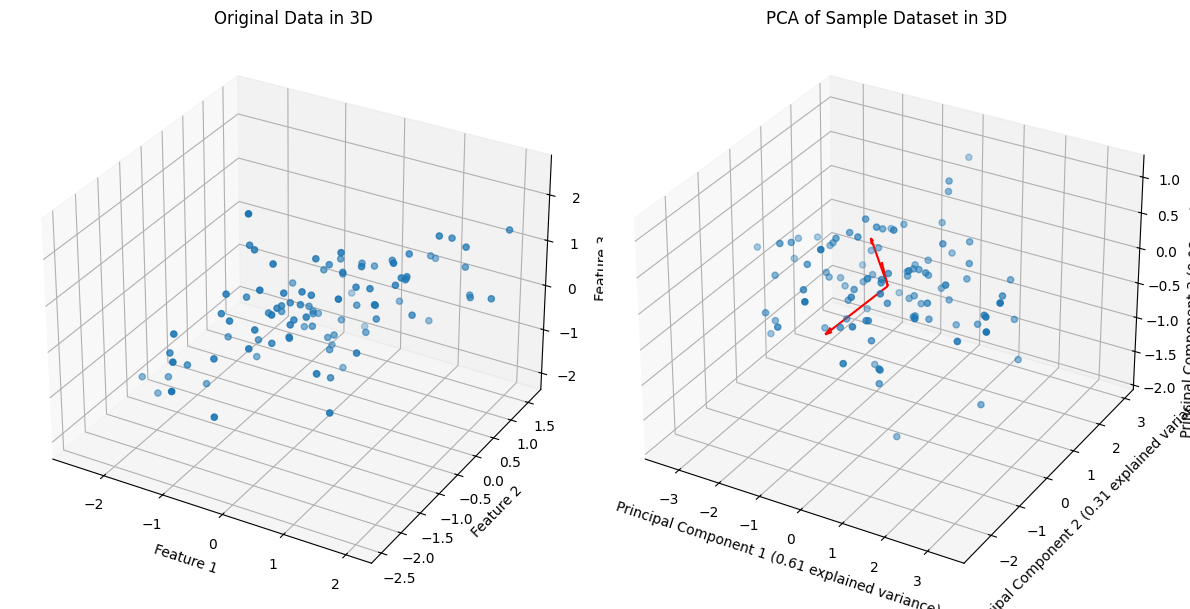
\includegraphics{images/pca_3d.png} 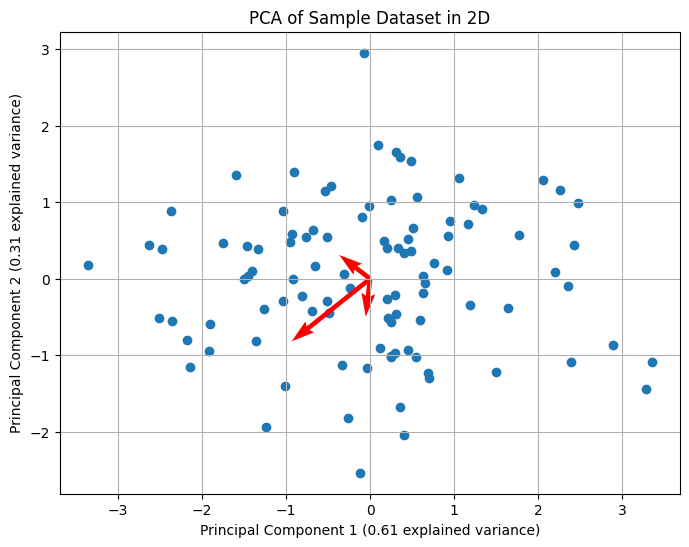
\includegraphics{images/pca_2d.png}
The red arrows in the plot represent the eigenvectors scaled by the
square roots of their respective eigenvalues. These vectors indicate the
directions of maximum variability in the data, which are the principal
axes determined by Principal Component Analysis (PCA). \textbf{Sources:}
- 2015\_Book\_AppliedMultivariateStatistical.pdf - ADM\_PCA.pdf
